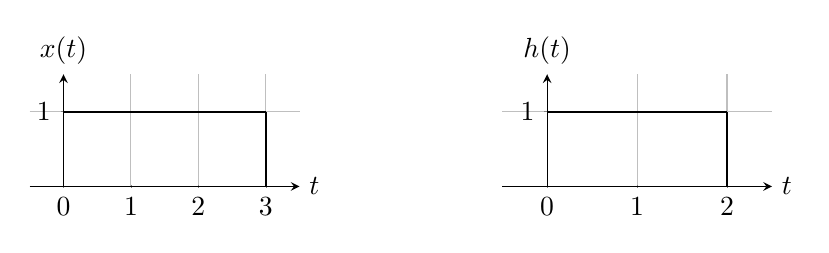
\begin{tikzpicture}
	\begin{axis}[
		xscale = 0.5,
		yscale = 0.25,
		xmin= -0.5, xmax = 3.5,
		ymin= 0, ymax = 1.5,
		axis x line=bottom,
		axis y line=center,
		xtick = {0,1,2,3},
		ytick = {1},
		xlabel=$t$, xlabel style={at={(ticklabel* cs:1)}, anchor= west},
		ylabel=$x(t)$, ylabel style={at={(ticklabel* cs:1)}, anchor=south},
		grid=both,
		]
		\addplot[domain=0:3, thick] (\x, 1);
        \draw[thick] (axis cs:3,0) -- (axis cs:3,1);
        \end{axis}
        
   	\begin{axis}[
    	xshift = 6cm,
		xscale = 0.5,
		yscale = 0.25,
		xmin= -0.5, xmax = 2.5,
		ymin= 0, ymax = 1.5,
		axis x line=bottom,
		axis y line=center,
		xtick = {0,1,2,3},
		ytick = {1},
		xlabel=$t$, xlabel style={at={(ticklabel* cs:1)}, anchor= west},
		ylabel=$h(t)$, ylabel style={at={(ticklabel* cs:1)}, anchor=south},
		grid=both,
		]
		\addplot[domain=0:2, thick] (\x, 1);
        \draw[thick] (axis cs:2,0) -- (axis cs:2,1);
        \end{axis}
        
\end{tikzpicture}